\section{Zielsetzung}
\label{sec:Zielsetzung}
Ziel des Versuchs ist es die Feldstärken unterschiedlicher Spulen in verschiedenen Anordnungen in
Abhängigkeit der Ortes zu messen. Weiterhin wird mit einer Ringspule ein Eisenkern magnetisiert und eine
Hystereskurve dazu aufgestellt.

\section{Theorie}
\label{sec:Theorie}
Im Allgemeinen erzeugen bewegte Ladungen magnetische Felder. Die magnetische Feldstärke ist eine vektorielle Größe
und ist durch das Biot-Savart-Gesetz
\begin{equation}
    \label{eqn:magFeldstaerke}
    \vec{H} = \mu_{0}\cdot\mu_{\symup{r}}\cdot \vec{B}
\end{equation}
gegeben. Dabei ist $\mu_{0}$ die Vakuumpermeabilität, $\mu_{\symup{r}}$ die materialabhängige relative
Permeabilität und $\vec{B}$ die magnetische Flussdichte. Die beiden Permeabilitäten lassen sich zu der gesamt
Permeabilität $\mu = \mu_0 \cdot \mu_{\symup{r}}$ zusammenfassen. Um die Magnetfeldstärken beliebiger
Leiterschleifen zu bestimmen, wird das Biot-Savart-Gesetz verwendet, das durch
\begin{equation}
    \label{eqn:biotsavart}
    \vec{B}(r) = \frac{\mu_{0}I}{4\pi} \int_{\Gamma} \frac{\vec{ds}\times \vec{r}}{r^3}
\end{equation}
bestimmt ist. $I$ ist in diesem Fall die Stromstärke und $\Gamma$ der Weg der Schleife. Für eine Spule mit
$n$ Windungen ergibt sich dann
\begin{equation}
    \label{eqn:nSpule}
    \vec{B}(x) = \frac{n \mu_0 I}{2} \frac{R^2}{(R^2 + x^2)^{\frac{3}{2}}} \cdot \hat{x}.
\end{equation}
$R$ ist dabei der Radius der Spule und $x$ ist der Abstand zum Spulenzentrum. Handelt es sich um eine
langgestreckte Spule mit Länge $l$, die auch Solenoid gennannt wird, lässt sich die Flussdichte durch
\begin{equation}
    \label{eqn:langeSpule}
    \vec{B}(x) = \mu_{\symup{r}}\mu_0 \frac{n}{l} I
\end{equation}
beschreiben, da die Feldlinien innerhalb der Spule parallel zur Spulenachse sind und das Feld homogen ist.
\autoref{eqn:langeSpule} gilt nur, wenn die Länge der Spule $l$ wesentlich kleiner als der Durchmesser $d$
der Spule ist. Für außerhalb der Spule lässt sich keine simple Formel bestimmen, da dort die Feldlinien
auffächern. Wird ein Solenoid nun zu einer Ringspule mit Radius $r_{\symup{T}} << l$ gebogen, fallen die
Randeffekte weg und die Flussdichte lässt sich nach \autoref{eqn:langeSpule} mit $l = 2\pi r_{\symup{T}}$
\begin{equation}
    \label{eqn:ringspule}
    \vec{B}(r) = \mu_{\symup{r}}\mu_0 \frac{n}{2\pi r_{\symup{T}}} I
\end{equation}
bestimmen. Damit ein homogenes Magnetfeld erzeugt wird, werden Helmholtz-Spulenpaare verwendet. Dazu werden
die zwei identische Spulen so positioniert, dass ihre Spulenachsen gleich sind und der Abstand der Zentren
gleich dem Spulenradius $R$ ist. Eine schematische Darstellung dafür ist in \autoref{fig:helmholtz} zu finden.
\begin{figure}
    \centering
    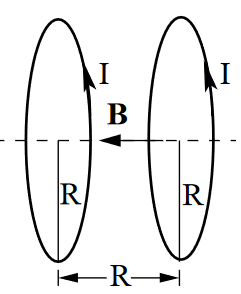
\includegraphics[scale=0.5]{helmholtzspulenpaar.png}
    \caption{Skizze eines Helmholtz-Spulenpaars \cite{sample}.}
    \label{fig:helmholtz}
\end{figure}
Die magnetische Flussdichte im Zentrum der Spule lässt sich durch das Biot-Savart-Gesetz bestimmen.
Die Gleichung für das Helmholtz-Spulenpaar ist dann durch Überlagerung der beiden Felder bestimmt.
Es ergibt sich
\begin{equation}
    \label{eqn:helmholtz}
    \vec{B}(x) = \frac{n\mu_0 I R^2}{(R^2+x^2)^{\frac{3}{2}}}.
\end{equation}

\subsection{Hystereskurve}
\label{sec:hysterese}
Befindet sich zusätzlich noch ein ferromagnetischer Stoff in der Spule muss dessen Magnetisierung $\vec{M}$
noch bedacht werden. Dieser Umstand lässt sich durch
\begin{equation}
    \vec{B} = \mu_0 (\vec{H} + \vec{M})
\end{equation}
ausdrücken. Ferromagnetische Stoffe haben so genannte Weiß'sche Bezirke in denen die magnetischen
Momente parallel zu einander ausgerichtet sind. In unmagnetisierten Materialien sind diese statistisch verteilt,
so dass ferromagnetische Stoffe ein permanentes magnetisches Moment besitzen.\\
Wird nun ein externes Magnetfeld angelegt richten sich die magnetischen Momente der Weiß'schen Bezirke
nach der Richtung des Magnetfelds aus bis das Gesamtfeld einen Sättigungswert
$B_{\symup{S}}$ erreicht. Wird das Magnetfeld nun abgeschaltet bleibt eine Restmagnetisierung
über, die Remanenz genannt wird. Um diese auszugleichen kann ein magnetisches Feld, das
auch Koerzitivkraft $H_{\symup{C}}$ genannt wird, aufgewandt werden. Nach weiterem Erhöhen des Gegenfelds
erreicht die Kurve den Sättigungswert $-B_[\symup{s}]$. Wird nun das Feld umgekehrt und erhöht, ergibt sich eine
symmetrische Kurve zum Ursprung, die schematisch in \autoref{fig:hysterese} dargestellt ist.
\begin{figure}[h]
    \centering
    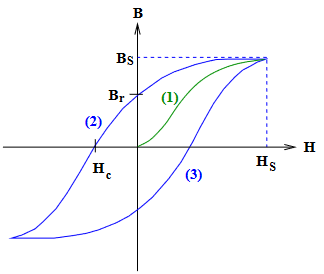
\includegraphics[scale=0.5]{hysterese.png}
    \caption{Schematische Darstellung einer Hystereskurve \cite{sample}.}
    \label{fig:hysterese}
\end{figure}
Diese Kurve heißt Hystereskurve und ist materialabhängig. Sie stellt den Zusammenhang zwischen magnetischer Feldstärke
$\vec{H}$ und relativer Permeabilität $\mu_{\symup{r}}$ dar.